% Generated by ic_study.analysis.v4_report_export from the v4 report with
% manifest SHA-256 6608b3960eb73011caca97870a4ffd3dbfbcd4c2df09bbbcb576c1c9452cf981.
% Edited during the journal revision (agent S, 2026-10-13): captions, headers and
% categorical cells in plain English; every number keeps its \resultnum binding.
\begin{figure*}[tp]
\centering
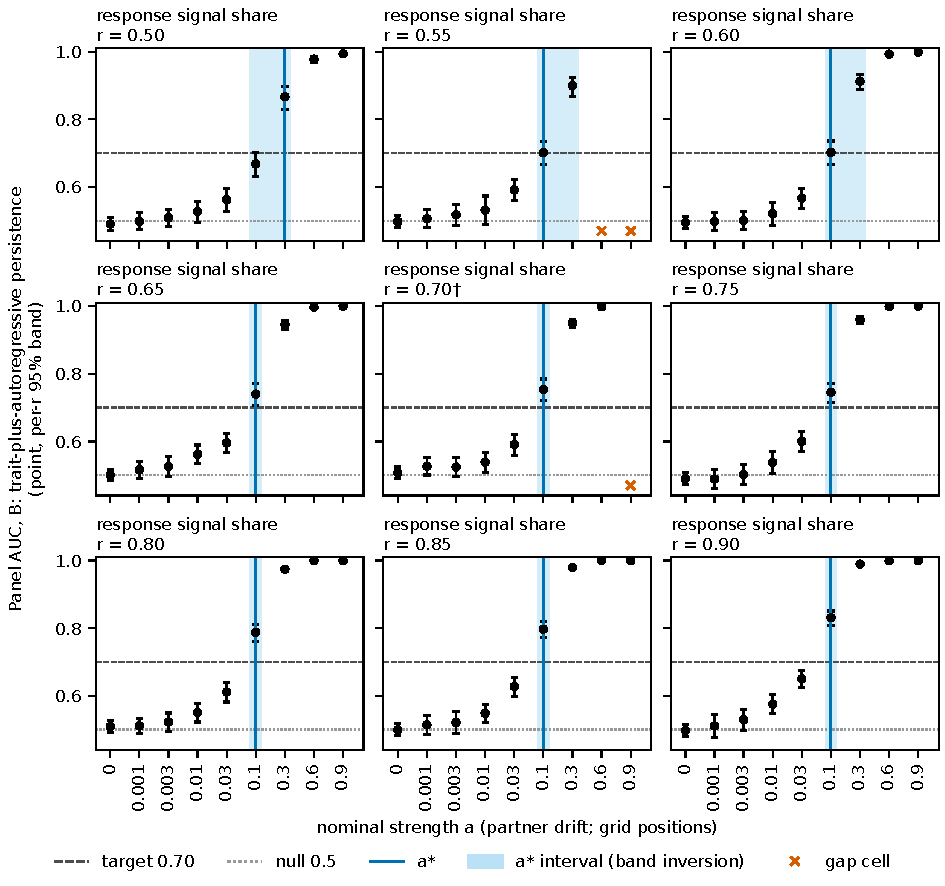
\includegraphics[width=\textwidth,height=175mm,keepaspectratio]{generated/F2_auc_profiles_B.pdf}
\caption{AUC profiles against B (trait plus autoregressive persistence), one panel per signal share $r$: point AUC and per-$r$ simultaneous 95\% band at each grid strength of the influence strength $a$ (ordinal positions), the primary target 0.70 (dashed), 0.5 (dotted), the first boundary $a^*$ (vertical line) and its interval (shaded). Crosses mark fit gaps. The band gives no joint coverage across $r$, models or channels.}\label{fig:v4-F2B}
\end{figure*}
